\documentclass[aspectratio=169,10pt]{beamer}

% Theme
\usetheme{Madrid}
\usecolortheme{default}
\setbeamertemplate{navigation symbols}{}
\setbeamertemplate{footline}[frame number]

% Packages
\usepackage{amsmath,amssymb}
\usepackage{booktabs}
\usepackage{tikz}
\usetikzlibrary{arrows.meta,positioning,shapes.geometric,calc}
\usepackage{algorithm2e}
\usepackage{xcolor}
\usepackage{graphicx}
\graphicspath{{images/}}

% Colors
\definecolor{boundary}{RGB}{220,53,69}
\definecolor{episode1}{RGB}{40,167,69}
\definecolor{episode2}{RGB}{0,123,255}
\definecolor{episode3}{RGB}{255,193,7}

% Title
\title{Unsupervised Episode Detection for Scene Graph Understanding}
\author{}
\date{}

\begin{document}

%==============================================================================
\begin{frame}
\titlepage
\end{frame}

% %==============================================================================
% \begin{frame}{Why Scene Graphs?}

% \textbf{Scene graphs}: Structured representation encoding entities, attributes, and relationships

% \vspace{0.3cm}
% \textbf{Key Benefits}:
% \begin{itemize}
% \item Enable \textbf{spatial and temporal reasoning} in multimodal settings
% \item Provide \textbf{grounding for LLMs} in embodied AI and robotics
% \item Bridge gap between visual perception and symbolic reasoning
% \item Support complex queries about actions, objects, and relationships
% \end{itemize}

% \end{frame}

%==============================================================================
\begin{frame}{Problem: Flat Scene Graphs Lack Structure}

\textbf{Scene graphs} represent video actions as sequences of triplets:
\begin{center}
\small
\texttt{[person, verb, pick-up], [pick-up, dobj, mop], [mop, from, floor], ...}
\end{center}

\vspace{0.2cm}
\textbf{Challenge}: Temporal reasoning requires understanding \textbf{episode boundaries}

\vspace{0.2cm}
\begin{columns}
\begin{column}{0.48\textwidth}
\textbf{Without hierarchy:}
\begin{itemize}
\item Flat sequence of 11 actions
\item No phase structure
\item Model must infer relationships
\end{itemize}
\end{column}
\begin{column}{0.48\textwidth}
\textbf{With hierarchy:}
\begin{itemize}
\item Episode 1: Prepare \& sweep
\item Episode 2: Store supplies
\item Episode 3: Retrieve from cabinet
\end{itemize}
\end{column}
\end{columns}

\vspace{0.2cm}
\textbf{Key Question}: How to detect meaningful phases \textit{without supervision}?

% \vspace{0.2cm}
% \textbf{Our Result}: Unsupervised episode detection improves SGQA accuracy from \textbf{20\% to 50\%} on hard temporal reasoning questions

\end{frame}

%==============================================================================
\begin{frame}{Background: Video Scene Graphs \& SGQA}

\begin{columns}
\begin{column}{0.45\textwidth}
\textbf{Video Scene Graph}
\begin{center}
\includegraphics[width=0.95\textwidth]{video_scene_graph_definition.png}
\end{center}
\scriptsize
\textbf{Structure}: \textbf{Agent} $\xrightarrow{\text{verb}}$ \textbf{Action} $\xrightarrow{\text{dobj}}$ \textbf{Object}\\
with \texttt{with}, \texttt{of}, \texttt{into} relations
\end{column}
\begin{column}{0.55\textwidth}
\textbf{SGQA Task}
\begin{center}
\includegraphics[width=0.95\textwidth]{SGQA_demo.png}
\end{center}
\scriptsize
Answer temporal reasoning questions:\\
``What was done \textit{before} X?'', ``After completing A...''
\end{column}
\end{columns}

\vspace{0.2cm}
\hfill\scriptsize Figures from Yang et al. (ACL 2025)

\end{frame}

%==============================================================================
\begin{frame}{Our Approach: EpiMine-inspired Episode Detection for Scene Graphs}

\textbf{Key Insight}: Episode boundaries occur where \textbf{co-occurrence patterns shift}

\vspace{0.3cm}
\begin{center}
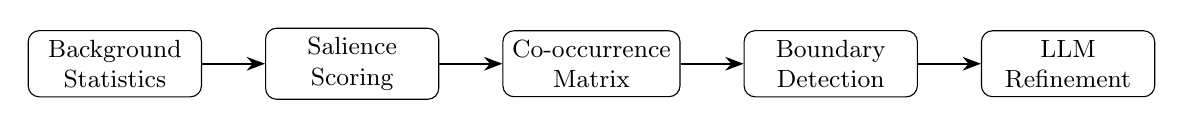
\begin{tikzpicture}[
    node distance=0.8cm,
    box/.style={rectangle, draw, rounded corners, minimum width=2.2cm, minimum height=0.7cm, align=center, font=\small},
    arrow/.style={-{Stealth}, thick}
]
\node[box] (bg) {Background\\Statistics};
\node[box, right=of bg] (sal) {Salience\\Scoring};
\node[box, right=of sal] (cooc) {Co-occurrence\\Matrix};
\node[box, right=of cooc] (bound) {Boundary\\Detection};
\node[box, right=of bound] (llm) {LLM\\Refinement};

\draw[arrow] (bg) -- (sal);
\draw[arrow] (sal) -- (cooc);
\draw[arrow] (cooc) -- (bound);
\draw[arrow] (bound) -- (llm);
\end{tikzpicture}
\end{center}

\vspace{0.3cm}
\textbf{Hybrid approach}:
\begin{itemize}
\item \textbf{Statistical}: Unsupervised boundary detection 
\item \textbf{Semantic}: LLM generates episode names/descriptions
\end{itemize}

\end{frame}

%==============================================================================
\begin{frame}{Step 1: Salience -- Identifying Discriminative Terms}

\textbf{Goal}: Find terms that characterize the current activity

\vspace{0.2cm}
\textbf{Formula}:
\[
\text{salience}(t) = \underbrace{(1 + \log(f_{\text{fg}})^2)}_{\text{foreground boost}} \times \underbrace{\log\left(\frac{N_{\text{bg}}}{f_{\text{bg}}}\right)}_{\text{IDF component}}
\]

\vspace{0.1cm}
\begin{itemize}
\item $f_{\text{fg}}$: term frequency in current sample (foreground)
\item $f_{\text{bg}}$: term frequency across all samples (background)
\end{itemize}

\vspace{0.2cm}
\begin{columns}
\begin{column}{0.55\textwidth}
\textbf{Example} (Car Cleaning):
\begin{center}
\small
\begin{tabular}{lcc}
\toprule
\textbf{Term} & \textbf{Salience} & \textbf{Interpretation} \\
\midrule
mop-stick & 18.86 & Highly discriminative \\
wall & 9.98 & Discriminative \\
person & $\approx 0$ & Common (filtered) \\
\bottomrule
\end{tabular}
\end{center}
\end{column}
\begin{column}{0.42\textwidth}
\colorbox{blue!10}{
\parbox{0.95\textwidth}{
\small
\textbf{Tunable: \texttt{min\_freq}}\\[0.1cm]
Filter terms with $f_{\text{fg}} < $ \texttt{min\_freq}\\[0.1cm]
\textit{Higher} $\rightarrow$ fewer episodes\\
\textbf{Optimal}: \texttt{min\_freq=2}
}}
\end{column}
\end{columns}

\end{frame}

%==============================================================================
\begin{frame}{Step 2: Co-occurrence Matrix}

\textbf{Goal}: Measure similarity between consecutive actions using top-$k$ salient terms

\vspace{0.2cm}
\textbf{Jaccard Similarity} (using only top-$k$ key terms):
\[
\text{cooccur}(A_i, A_j) = \frac{|\text{terms}_k(A_i) \cap \text{terms}_k(A_j)|}{|\text{terms}_k(A_i) \cup \text{terms}_k(A_j)|}
\]

\vspace{0.2cm}
\begin{columns}
\begin{column}{0.55\textwidth}
\textbf{Intuition}:
\begin{itemize}
\item \textbf{High co-occurrence} $\rightarrow$ same episode
\item \textbf{Low co-occurrence} $\rightarrow$ boundary
\end{itemize}

\vspace{0.2cm}
\begin{center}
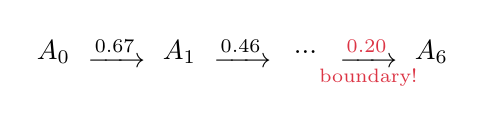
\begin{tikzpicture}[scale=0.8]
\node at (0,0) {$A_0$};
\node at (1.0,0) {$\xrightarrow{0.67}$};
\node at (2.0,0) {$A_1$};
\node at (3.0,0) {$\xrightarrow{0.46}$};
\node at (4.0,0) {...};
\node at (5.0,0) {$\xrightarrow{\textcolor{boundary}{0.20}}$};
\node at (6.0,0) {$A_6$};
\node[font=\scriptsize,text=boundary] at (5.0,-0.4) {boundary!};
\end{tikzpicture}
\end{center}
\end{column}
\begin{column}{0.42\textwidth}
\colorbox{blue!10}{
\parbox{0.95\textwidth}{
\small
\textbf{Tunable: \texttt{top\_k}}\\[0.1cm]
Limit to top-$k$ salient terms\\[0.1cm]
\texttt{topk=all}: noisy (18.3\% avg)\\
\texttt{topk=5}: too sparse (20.8\%)\\
\textbf{Optimal}: \texttt{topk=10} (24.2\%)
}}
\end{column}
\end{columns}

\end{frame}

%==============================================================================
\begin{frame}{Step 3: Boundary Detection}

\begin{columns}
\begin{column}{0.55\textwidth}
\textbf{Algorithm}:
\begin{enumerate}
\item Compute consecutive scores: $s_i = \text{cooccur}(A_i, A_{i+1})$
\item Calculate threshold: $\tau = \mu - t \cdot \sigma$
\item If $s_i < \tau$: start new episode
\end{enumerate}

\vspace{0.2cm}
\textbf{Example} (11 actions):
\begin{center}
\scriptsize
\begin{tabular}{cccccc}
\toprule
$A_0{\to}A_1$ & ... & $A_5{\to}A_6$ & ... & $A_9{\to}A_{10}$ \\
\midrule
0.67 & ... & \textcolor{boundary}{\textbf{0.20}} & ... & \textcolor{boundary}{\textbf{0.31}} \\
\bottomrule
\end{tabular}
\end{center}

$\tau = 0.437 - 1.0 \times 0.129 = 0.308$
\end{column}
\begin{column}{0.42\textwidth}
\colorbox{blue!10}{
\parbox{0.95\textwidth}{
\small
\textbf{Tunable: \texttt{threshold\_std}}\\[0.1cm]
Formula: $\tau = \mu - t \cdot \sigma$\\[0.1cm]
Lower $t$ $\rightarrow$ more boundaries\\
Higher $t$ $\rightarrow$ fewer episodes\\[0.1cm]
\begin{tabular}{lcc}
\scriptsize $t$ & \scriptsize Avg & \scriptsize Max \\
\scriptsize 1.0 & \scriptsize 15.8\% & \scriptsize 30\% \\
\scriptsize \textbf{1.5} & \scriptsize \textbf{24.2\%} & \scriptsize \textbf{50\%} \\
\scriptsize 2.0 & \scriptsize 23.3\% & \scriptsize 30\% \\
\end{tabular}
}}
\end{column}
\end{columns}

\vspace{0.2cm}
\textbf{Detected Episodes}:
\begin{itemize}
\item \textcolor{episode1}{Episode 0}: Actions [0-5] -- pick-up, sweep, close, place, open, put
\item \textcolor{episode2}{Episode 1}: Actions [6-9] -- move, open, pick-up, move
\item \textcolor{episode3}{Episode 2}: Action [10] -- pick
\end{itemize}

\end{frame}

%==============================================================================
\begin{frame}[fragile]{Step 4: LLM Refinement}

\textbf{LLM refines boundaries into structured episodes}:

\vspace{0.1cm}
\begin{columns}
\begin{column}{0.55\textwidth}
\small
\begin{verbatim}
{
  "episode_id": 0,
  "name": "Prepare and Sweep",
  "description": "Pick up mop,
    sweep floor, manage door",
  "core_structure": {
    "agent": "person",
    "actions": ["pick-up","sweep"],
    "objects": ["mop-stick","floor"]
  },
  "time": {
    "action_indices": [0,1,2,3,4,5],
    "duration": 6
  }
}
\end{verbatim}
\end{column}
\begin{column}{0.42\textwidth}
\colorbox{blue!10}{
\parbox{0.95\textwidth}{
\small
\textbf{Tunable: \texttt{use\_llm}, \texttt{gen\_model}}\\[0.1cm]
\texttt{use\_llm=0}: structural only\\
\texttt{use\_llm=1}: semantic naming\\[0.1cm]
\texttt{gen\_model}: gpt5-mini vs gpt5\\[0.1cm]
\begin{tabular}{lcc}
\scriptsize Setting & \scriptsize Avg & \scriptsize Max \\
\scriptsize noLLM & \scriptsize 18.9\% & \scriptsize 30\% \\
\scriptsize \textbf{LLM} & \scriptsize \textbf{23.3\%} & \scriptsize \textbf{50\%} \\
\end{tabular}\\[0.1cm]
\textit{+4.4\% avg improvement}
}}
\end{column}
\end{columns}

\vspace{0.2cm}
\textbf{Output}: Episode name, description, core structure, temporal info, discriminative terms

\end{frame}

%==============================================================================
\begin{frame}{Experiments: Hard-10 Benchmark}

\textbf{Motivation}: General SGQA accuracy (88.6\%) may hide weaknesses on hard cases

\vspace{0.2cm}
\begin{columns}
\begin{column}{0.55\textwidth}
\textbf{Hard-10 Construction}:
\begin{enumerate}
\item Run GPT-5 on full SGQA (500 questions)
\item Identify \textbf{88 questions} where GPT-5 failed
\item Select \textbf{first 10} for hyperparameter tuning
\end{enumerate}

\vspace{0.2cm}
\textbf{Hard Question Categories}:
\begin{center}
\small
\begin{tabular}{lc}
\toprule
\textbf{Category} & \textbf{Count} \\
\midrule
temporal\_ordering & 57 \\
multi\_step & 17 \\
both\_hands & 9 \\
\bottomrule
\end{tabular}
\end{center}
\end{column}
\begin{column}{0.42\textwidth}
\colorbox{blue!10}{
\parbox{0.95\textwidth}{
\small
\textbf{Grid Search}\\[0.1cm]
$3 \times 2 \times 3 \times 2 = 36$ configs\\[0.1cm]
\begin{tabular}{ll}
\scriptsize threshold\_std & \scriptsize 1.0, 1.5, 2.0 \\
\scriptsize min\_freq & \scriptsize 1, 2 \\
\scriptsize top\_k & \scriptsize 5, 10, all \\
\scriptsize use\_llm & \scriptsize 0, 1 \\
\end{tabular}\\[0.2cm]
\textbf{Baseline}: 20\% (2/10)
}}
\end{column}
\end{columns}

\end{frame}

%==============================================================================
\begin{frame}{Results: Grid Search on Hard-10}

\begin{columns}
\begin{column}{0.55\textwidth}
\textbf{Best Configurations}:
\begin{center}
\begin{tabular}{ccccc}
\toprule
\textbf{Acc} & \textbf{$t$} & \textbf{mf} & \textbf{topk} & \textbf{LLM} \\
\midrule
\textcolor{episode1}{\textbf{50\%}} & 1.5 & 2 & 10 & Yes \\
\textcolor{episode2}{\textbf{40\%}} & 1.5 & 2 & 5 & Yes \\
30\% & various & various & 5,10 & mixed \\
\midrule
20\% & \multicolumn{4}{c}{Baseline (no episodes)} \\
\bottomrule
\end{tabular}
\end{center}

\vspace{0.2cm}
\textbf{Key findings}:
\begin{itemize}
\item \textbf{+150\% relative improvement} (20\% $\rightarrow$ 50\%)
\item Top configs share: $t$=1.5, mf=2, LLM=yes
\item Parameter interactions matter
\end{itemize}
\end{column}
\begin{column}{0.42\textwidth}
\textbf{Parameter Impact}:
\small
\begin{tabular}{lcc}
\toprule
\textbf{Parameter} & \textbf{Best} & \textbf{Why} \\
\midrule
$t$ & 1.5 & Moderate sensitivity \\
mf & 2 & Filter noise \\
topk & 10 & Focus key terms \\
LLM & yes & +4.4\% avg \\
\bottomrule
\end{tabular}

\vspace{0.2cm}
\colorbox{blue!10}{
\parbox{0.95\textwidth}{
\small
\textbf{topk ablation}\\[0.1cm]
\begin{tabular}{lcc}
\scriptsize all & \scriptsize 18.3\% & \scriptsize noisy \\
\scriptsize 5 & \scriptsize 20.8\% & \scriptsize sparse \\
\scriptsize \textbf{10} & \scriptsize \textbf{24.2\%} & \scriptsize balanced \\
\end{tabular}
}}
\end{column}
\end{columns}

\end{frame}

%==============================================================================
\begin{frame}{Results: Full SGQA \& Analysis}

\begin{columns}
\begin{column}{0.48\textwidth}
\textbf{Full SGQA} (500 questions)
\begin{center}
\small
\begin{tabular}{lcc}
\toprule
\textbf{Method} & \textbf{EM} & \textbf{$\Delta$} \\
\midrule
Baseline & 88.6\% & -- \\
EpiMine (gpt5-mini) & 89.6\% & +1.0\% \\
EpiMine (gpt5) & \textbf{90.6\%} & \textcolor{episode1}{+2.0\%} \\
\bottomrule
\end{tabular}
\end{center}

\vspace{0.2cm}
\textbf{Hard-10} (10 questions)
\begin{center}
\small
\begin{tabular}{lcc}
\toprule
\textbf{Method} & \textbf{EM} & \textbf{$\Delta$} \\
\midrule
Baseline & 20\% & -- \\
EpiMine (gpt5-mini) & \textbf{50\%} & \textcolor{episode1}{+30\%} \\
EpiMine (gpt5) & 40\% & +20\% \\
\bottomrule
\end{tabular}
\end{center}
\end{column}
\begin{column}{0.48\textwidth}
\textbf{LLM Impact Analysis}:
\begin{center}
\small
\begin{tabular}{lccc}
\toprule
\textbf{Config} & \textbf{noLLM} & \textbf{+LLM} & \textbf{$\Delta$} \\
\midrule
$t$=1.5, topk=10 & 20\% & \textbf{50\%} & \textcolor{episode1}{+30\%} \\
$t$=1.5, topk=5 & 10\% & \textbf{40\%} & \textcolor{episode1}{+30\%} \\
\midrule
$t$=1.0, topk=10 & 30\% & 10\% & \textcolor{boundary}{-20\%} \\
\bottomrule
\end{tabular}
\end{center}

\vspace{0.2cm}
\textbf{Insight}: LLM amplifies good boundaries, but can hurt poor segmentation

\vspace{0.2cm}
\colorbox{blue!10}{
\parbox{0.95\textwidth}{
\small
\textbf{Takeaway}: Larger gains on harder questions; model choice is task-dependent
}}
\end{column}
\end{columns}

\end{frame}

% %==============================================================================
% \begin{frame}{Summary \& Future Directions}

% \textbf{Contributions}:
% \begin{enumerate}
% \item \textbf{EpiMine}: Unsupervised episode detection via co-occurrence pattern shifts
% \item \textbf{Hybrid approach}: Statistical boundaries + LLM semantic refinement
% \item \textbf{Hard-10 benchmark}: Focused evaluation on difficult temporal reasoning
% \end{enumerate}

% \vspace{0.2cm}
% \textbf{Results}: 88.6\% $\rightarrow$ 90.6\% on SGQA; \textbf{20\% $\rightarrow$ 50\%} on Hard-10

% \vspace{0.3cm}
% \textbf{Future Directions}:
% \begin{columns}
% \begin{column}{0.32\textwidth}
% \textbf{Hierarchical structure}
% \begin{itemize}
% \item Nested episodes
% \item Scene-level abstraction
% \end{itemize}
% \end{column}
% \begin{column}{0.32\textwidth}
% \textbf{Multimodal integration}
% \begin{itemize}
% \item Visual features
% \item Grounded boundaries
% \end{itemize}
% \end{column}
% \begin{column}{0.32\textwidth}
% \textbf{Long-form video}
% \begin{itemize}
% \item Hour-long videos
% \item Multi-hop reasoning
% \end{itemize}
% \end{column}
% \end{columns}

% \end{frame}

\end{document}
